% \chapter{Motion Deblurring using Partially-Coherent Coded Illumination}

\section{High-Throughput Imaging}
Throughput is a primary concern for many imaging applications - for example, the clinical laboratory a large hospital may need to scan hundreds of histology slides per hour. Often, slide imaging or scanning large samples at high resolution requires the registration and tiling of many images acquired using a high-magnification objective. The acquisition of these datasets is often very long, owing to the precise positioning required as well as a necessary autofocusing step prior to each acquisition. Optimization of this process would clearly benefit hospitals and research centers studying datasets which necessitate a large field of view with high resolution.

Most modern high-throughput imaging systems use a stop-and-stare imaging style, where images are acquired by moving the sample to many positions, stopping, autofocusing, and finally acquiring an image. The full-field image is then stitched together using a registration algorithm. As mentioned previously, this method is often prohibitively slow due to the time necessary to stop and start the motion as well as autofocusing. A promising alternative to this scheme is strobed illumination, where the sample is moved constantly while the illumination is strobed, or flashed once each exposure using a very short, high-intensity pulse width. In this framework the image is still blurred, but the blurring is designed to be smaller than the system PSF causing no image degradation.

\section{Motion Deblur}

Strobed illumination is an ideal implementation in many applications. However, producing a very bright, very short pulse can often be difficult, particularly when a sample is moving fast, or in a low-resource setting such as a portable device where illumination power and intensity are restrcted. A promising alternative to strobed illumination is motion compensation using a deblurring algorithm which incorporates hardware coding techniques. Non-blind motion deblurring was previously explored in the context of computational photography, including several hardware implementations which exploit multiple cameras \cite{nayarDeblur, CaiDeblurring} or coded exposures \cite{raskar2006coded}. In addition, blind deblurring for photography has been extensively studied in the context of computational photography, where priors such as object statistics \cite{fergus2006removing, Shan:2008:HMD:1360612.1360672,Cho:2009:FMD:1618452.1618491,levin2006blind} and wavelet sparsity \cite{caiWavelet} to solve for the blur kernel and latent image simultaneously. In general, in-plane motion blur can be modeled as the convolution of a static intensity image ($I_s$) with a blur kernel $B$, which defines the smearing of a single point as it is moved across the field of view during a single exposure:

\begin{equation}\label{blurForwardModel}
I_{blurred}  (\vec{r})= I_0(\vec{r}) *  B(\vec{r})
\end{equation}

Here $\vec{r}$ and $\vec{k}$ represent the spatial coordinates and the Fourier conjugate variables for k-space respectively, and $I_0$ is the unblurred image of the sample or scene. In this simple case, we assume complete knowledge of the blur kernel $B$. The inverse problem can be formulated as a simple deconvolution of the static intensity image:

\begin{equation}\label{eq:blurInverseModel}
\tilde I_0 (\vec{r}) = \mathscr{F}^{-1}_{2D} \{\frac{I_{blurred}}{ \tilde{B}(\vec{k})}\}
\end{equation}

Where $\tilde{\cdot}$ denotes the 2D Fourier Transform. This inverse problem is a standard deconvolution problem and can be solved using a single least squares operation. Like most deconvolution problems, this problem is ill-posed and requires regularization to solve due to small values or zeros in the spectrum of $B$. This regularizer can be tailored to the problem using a-priori information about the sample, but in general a $\ell_2$ regularizer provides adequate results, and allows a single-step solution for a general object.

In many cases we not only know $B$ a priori, but have complete control over the shape of $B$ subject to practical hardware constraints. We can, therefore, choose an optimal motion pathway as well as illumination or exposure magnitude before acquiring to enhance the quality of our reconstructions. In the case where exposure is not coded, $B$ is simply a 1D \textit{rect} function placed into a 2D image as shown in Fig. \ref{fig:deblur}. In the Fourier domain, this transforms to a \textit{sinc} function, which has many zero crossings, making it hard to invert even if $B$ is perfectly known. The problem of designing an optimal $B$ motivated the design of the flutter-shutter camera \cite{raskar2006coded}. In this design, a ferrite shutter was placed in front of a camera lens and was opened and closed repeatedly during a single camera exposure. As a sample moves across the field it is convolved with this shutter time series, mapped to the spatial dimension by the velocity of the object, which is assumed to be known. This allows the user to optimize the blur kernel based on the object's velocity and exposure time.

A common metric for the fitness of a particular choice of $B$ is the condition number $\kappa$.  Generally, the condition number is the ratio of the larges to smallest singular value of the filter $H$. For linear shift-invariant (LSI) systems these are equal to the absolute value of the maximum and minimum Fourier coefficients respectively:

\begin{equation}\label{condNum}
 \kappa\{B\} = \frac{\sigma_{max}\{B\}}{\sigma_{min}\{B\}} = ||B||_p || B^{-1}||_p = \frac{\max{|\tilde{B}(\vec{k})|}}{\min{|\tilde{B}(\vec{k})|}}
\end{equation}

This metric can be evaluated quickly which makes optimizing $B$ directly numerically feasible. Essentially, this metric promotes a flat Fourier spectrum of $B$ and penalizes values close to zero, which makes the problem well-posed. It is important to note that the optimum solution of $B$ is clearly a delta function $\delta(\vec{r})$, and this optimization will converge to this solution if left unconstrained. However, a delta function corresponds to strobed illumination, which provides much less overall exposure, and therefore a much noisier image compared to constant exposure. To counter this, we place a box constraint on the maximum intensity of the illumination, which has practical motivations based on the maximum illumination intensity. In practice we bound $B\in[0,1]$. In addition we place a constraint on the total illumination throughput of the system during an exposure time, $\sum_{\vec{r}} B(\vec{r})\geq \gamma$, where $\gamma$ is typically set to 50$\%$ of the maximum intensity to allow the algorithm reasonable freedom as in \cite{raskar2006coded}. The complete problem is expressed as:

\begin{equation}
\label{eq:deblurKernelProb}
\begin{aligned}
& \underset{B}{\text{minimize}}
& & \kappa \{ B \} = \frac{\max{|\tilde{B}(\vec{k})|}}{\min{|\tilde{B}(\vec{k})|}} \\
& \text{subject to}
& & \sum_{n=1}^N B[n] \geq \gamma N, \hspace{15pt} 0 \leq B[n] \leq 1 \hspace{5pt} \forall n
\end{aligned}
\end{equation}


Figure \ref{fig:deblur} shows example blur kernels with their representations in real space and Fourier space. Noise also plays an important role, as noise will corrupt spatial frequencies which have poor transmission, further motivating the design of kernels with a flat Fourier spectrum. This method was also applied to microscopy using programmable LED array illumination which allows motion deblurring by varying the intensities of the LED array during exposure times \cite{Ma:15}. Unlike the ferro-electric shutter used in \cite{raskar2006coded}, the LED array has no moving parts, which allows faster update speeds, and can provide coded multi-color illumination if tri-color LEDs are used.


\begin{figure}[ph]
\centering
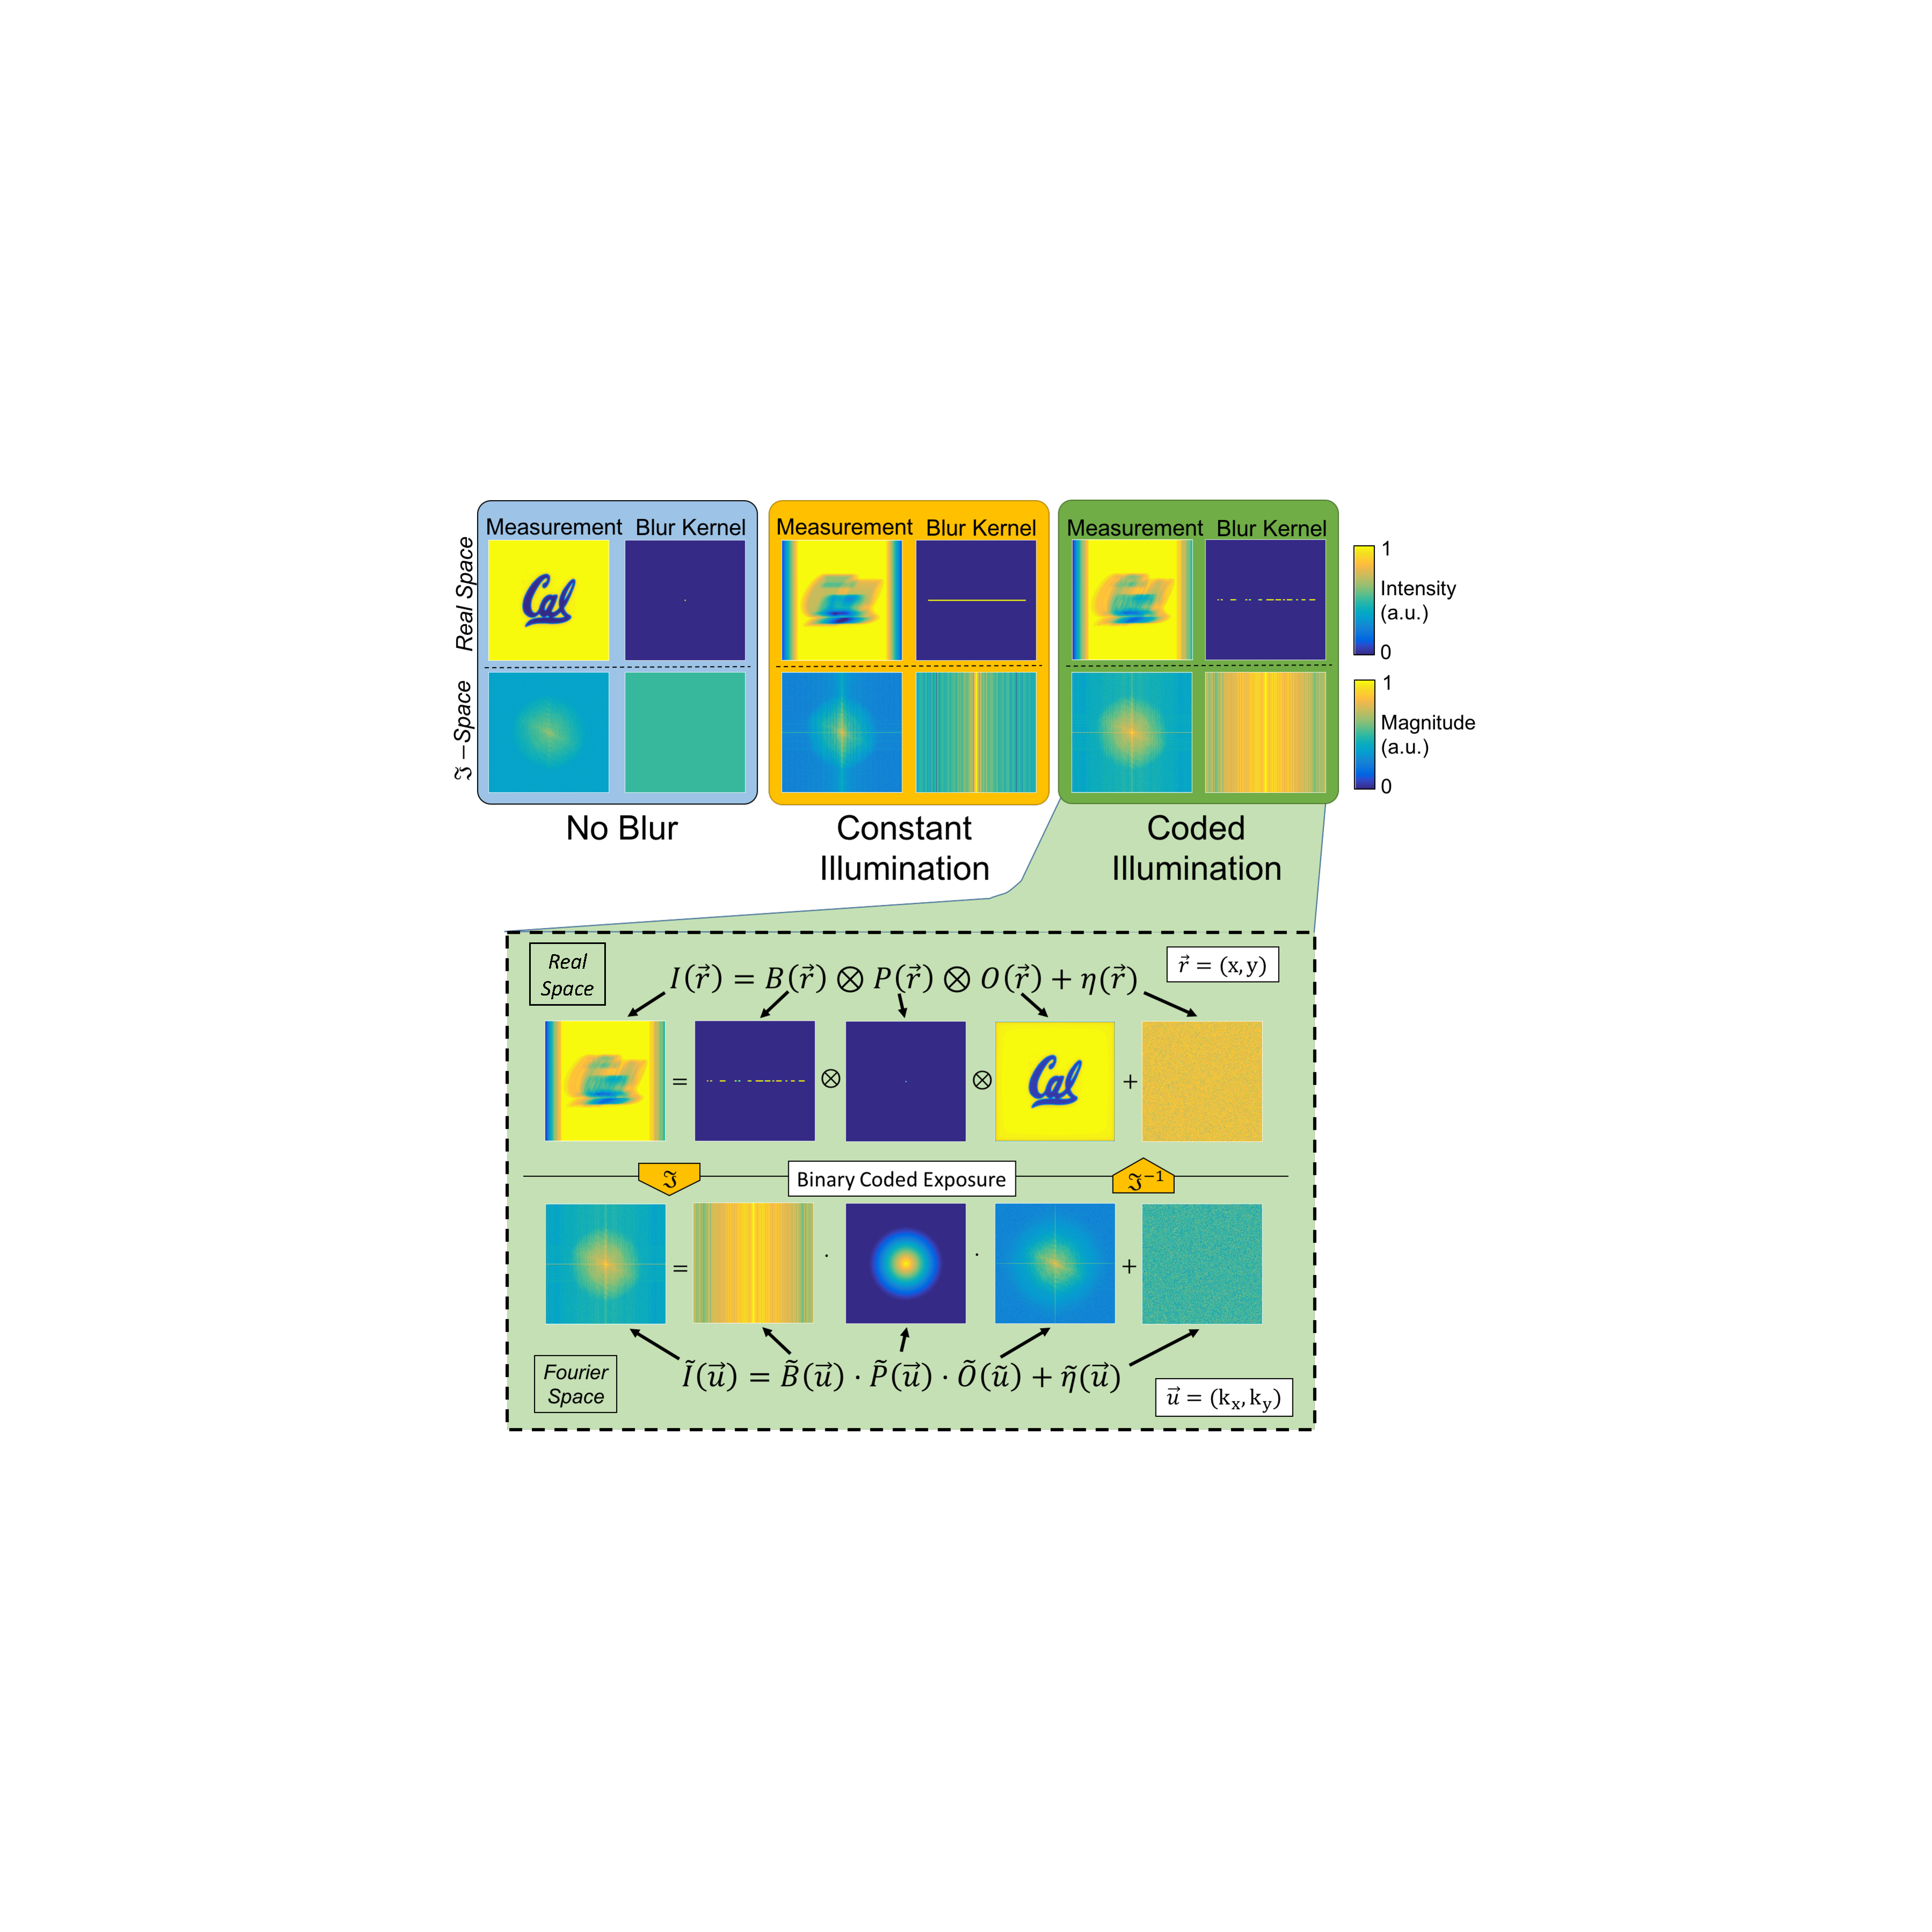
\includegraphics[width=1\textwidth]{deblur-fig1.pdf}
\caption{\label{fig:deblur}
Motion blur real-space and Fourier space representations. In the case of a static object, the object is filtered by the optical transfer function (OTF), assuming incoherent illumination. With motion blur, an additional convolution with a blurring function $B(\vec{r})$ causes attenuation in the frequency domain which acts as a cascaded linear filter on the object. In the case of coded blur, the transfer function is attenuated much less than in the conventional blur case. The colorbars are constant for real and fourier domain images respectively.}
\end{figure}

\section{Phase Imaging with Motion Deblur}
Phase Imaging using the Weak Object Transfer Function (WOTF) is highly compatible with motion deblur since both are modeled as linear convolutions on the same object. Chronologically, the results presented in Chapter 2 originated from the motion deblur problem, since we desired a method of recovering a blurred phase object from a single image. Recovering phase from multiple exposures is not considered in this chapter, but could be incorporated in future work. Our forward model in the frequency domain is a combination of the existing motion deblur model with the WOA. In the case of a single image, we model the blurred Intensity image as two separate convolutions, applied sequentially:

\begin{equation}
\tilde{I} = B * [ H_{\mu} * A + H_{\phi} * \phi]
\end{equation}

We can express the above equation as a block-wise matrix product in the Fourier domain, letting $\tilde{B}$, $\tilde{H}_{\mu}$, and $\tilde{H}_{\phi} $ be the diagonalized Fourier Transforms of the transform functions, and $\tilde{I}$, $\tilde{\mu}$, $\tilde{\phi}$ be the vectorized image and object components respectively:

\begin{equation}\label{forwardModelSingle}
\tilde{I} = \tilde{B} \cdot \begin{bmatrix} \tilde{H}_{\mu} & \tilde{H}_{\phi}\end{bmatrix}  \begin{bmatrix}\tilde{\mu}\\ \tilde{\phi} \end{bmatrix}
\end{equation}

The WOTF equations, which were defined in Chapter 2, are provided here again for a given illumination wavelength $\lambda $:

\begin{equation}\label{WOTFre_2}
\tilde{H}_{\mu}(\vec{f},\lambda) = \left[  P(\vec{f},\lambda) \star (P(\vec{f},\lambda)\cdot S(-\vec{f},\lambda))+ (P(\vec{f},\lambda) \cdot S(-\vec{f},\lambda)) \star P(\vec{f},\lambda)\right]
\end{equation}

\begin{equation}\label{WOTFim_2}
\tilde{H}_{\phi}(\vec{f},\lambda) = \frac{\lambda_0}{\lambda}\cdot\left[ P(\vec{f},\lambda) \star (P(\vec{f},\lambda)\cdot S(-\vec{f},\lambda))- (P(\vec{f},\lambda) \cdot S(-\vec{f},\lambda)) \star P(\vec{f},\lambda) \right],
\end{equation}

Combining measurements from the three color channels, we model the full over-determined system as:

\begin{equation}\label{forwardModel}
\begin{bmatrix}
\tilde{I}_{R}\cr \tilde{I}_{G}\cr \tilde{I}_{B}
\end{bmatrix}
= \begin{bmatrix}\tilde{B}_R & 0 & 0\cr 0 & \tilde{B}_G & 0 \cr 0 & 0 & \tilde{B}_B \end{bmatrix}
\times
\begin{bmatrix}\tilde{H}_{\mu,R} & \tilde{H}_{\phi,R}\cr \tilde{H}_{\mu,G} & \tilde{H}_{\phi,G}\cr \tilde{H}_{\mu,B} & \tilde{H}_{\phi,B}\end{bmatrix}
\times
 \begin{bmatrix}\tilde{\mu}\\ \tilde{\phi}\end{bmatrix}
\end{equation}.

As in \cite{raskar2006coded} and \cite{Ma:15}, we design our patterns such that the condition number of the blur kernel is minimized. By combining both motion deblurring and the linearized phase retrieval technique described in Chapter 2 (Eq. \ref{eq:Ha}, \ref{eq:Hp}), we can use knowledge of our WOTF as derived previously to influence our choice of $B$ to improve our overall phase and amplitude reconstruction from blurred data. The motion deblur problem as presented here will always degrade the result even with an ideal $B$ due to the constraints placed on the optimization problem. In the previous case, degradation due to the blurring operation was minimized by solving for a blur kernel with an optimally flat Fourier spectrum. This method, however, did not take into account the additional attenuation due to the OTF of the optical system.

\begin{figure}[h]
\centering
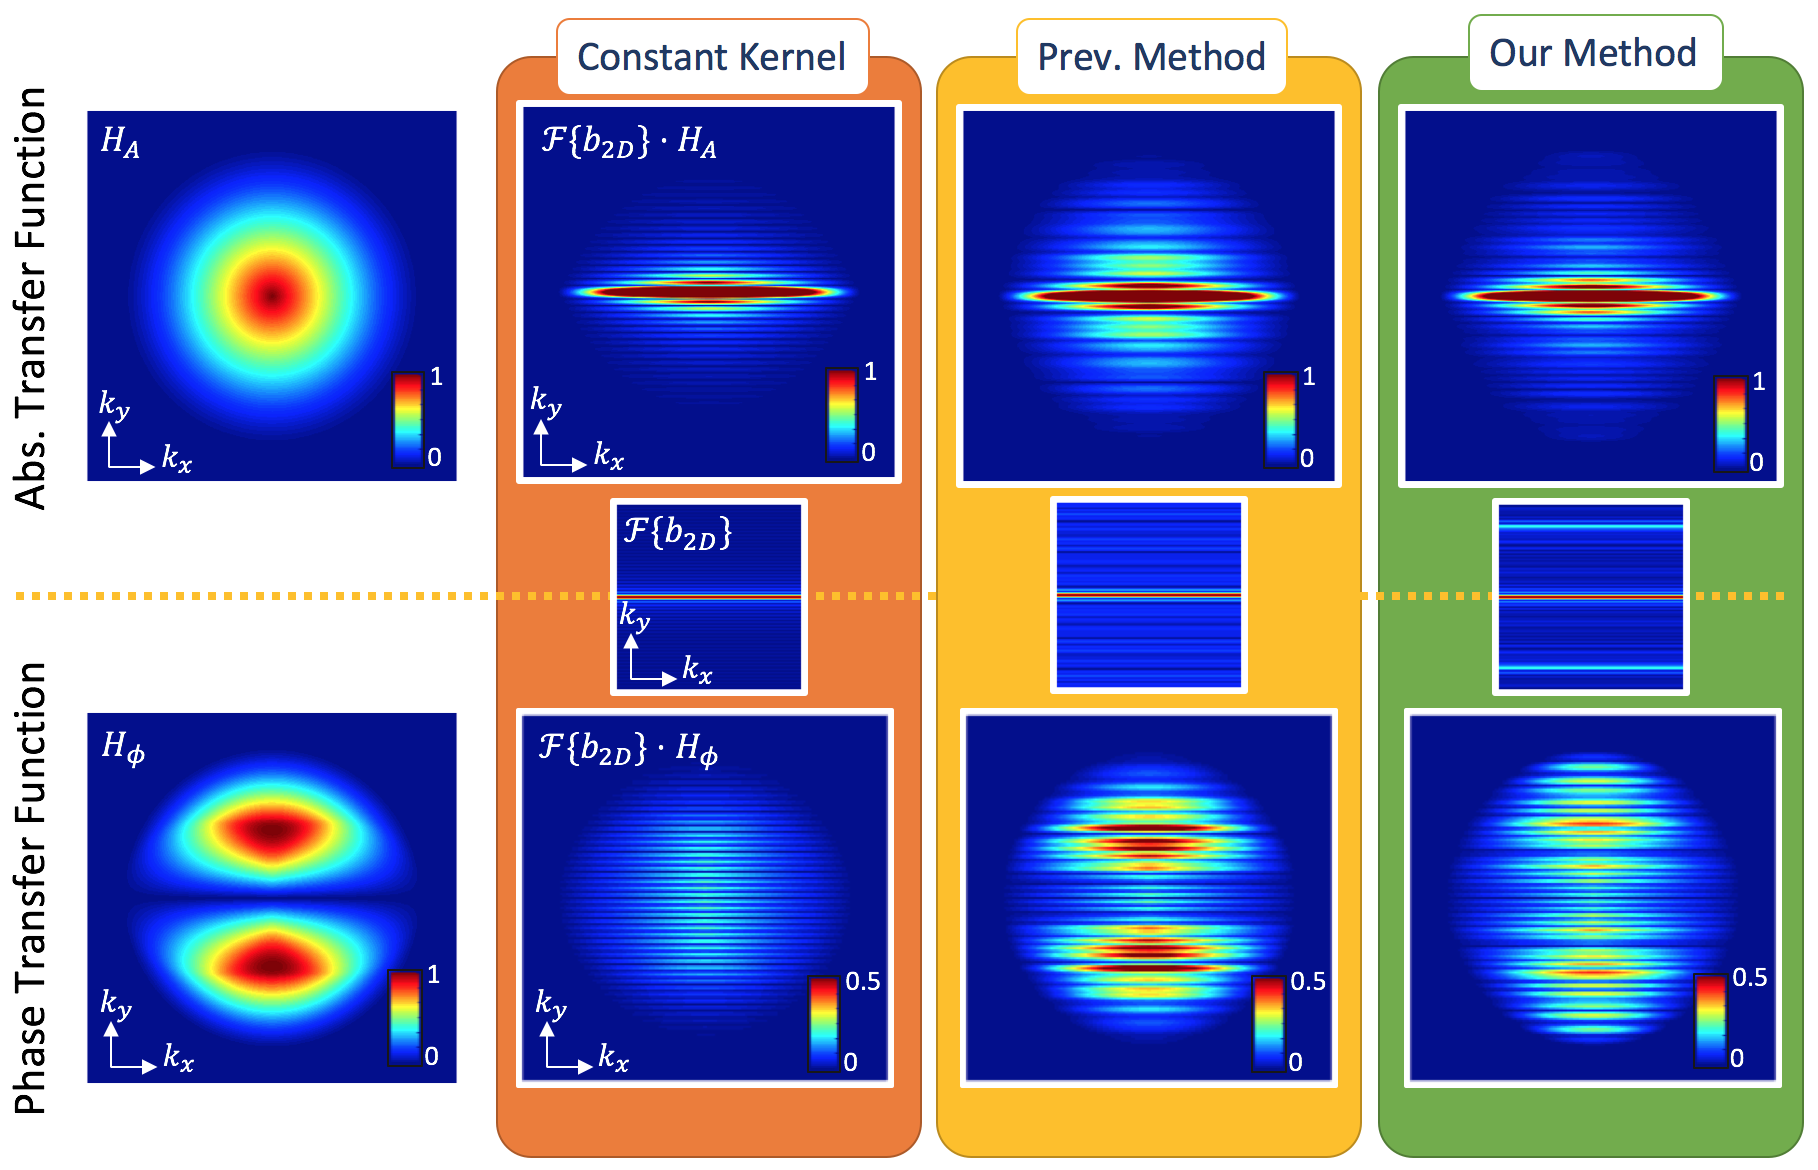
\includegraphics[width=1\textwidth]{deblur-fig2b.png}
\caption{\label{fig:deblurKernels}
Motion blurring kernels for 1D motion in the Fourier Domain.  \textbf{Left Column:} Unblurred absorption (top) and phase (bottom) transfer functions. \textbf{$2^{nd}$ Column}: Middle: Fourier transform of constant (non-coded) blur kernel. The top and bottom spectra in this column are the product of the unblurred transfer function and this center spectrum. \textbf{$3^{rd}$ Column}: Blurred transfer function spectra for temporal coding which does not consider WOTF structure. \textbf{$4^{th}$ Column}: Blurred transfer function spectra for temporal coding which emphasizes low and high frequencies based on WOTF structure.}
\end{figure}

Our improvement to the methods described in \cite{raskar2006coded} and \cite{Ma:15} is to consider the spectrums of cascaded filters in our system when designing our blur kernel. We can think of our sequential deconvolution problem as a single-step deconvolution which inverts the element-wise product of the blur kernel and WOTF's in the Fourier Domain. Therefore, the relative attenuation produced by the blur kernel at each frequency can be matched to reduce the degradation to highly attenuated frequencies in the WOTF, such as high frequencies in both amplitude and phase WOTF's, as well as low frequencies in the phase WOTF. The exact structure of this transfer function depends on the  pupil function of the optical system and design of the source. In practice, we note that the phase transfer function is of higher order than the amplitude transfer function (OTF), which generally means there are more zero crossings and values close to zero in the phase transfer function. Therefore, we will use the phase transfer function for optimizing the blur kernel.

To solve for the optimal blur kernel considering the WOTF, we modify Eq. \ref{eq:deblurKernelProb} to consider a 1D spectral reference $q$, which provides a measure of the attenuation imposed by the optical system at each spatial frequency in the blur kernel.

\begin{equation}
\begin{aligned}
& \underset{B}{\text{minimize}}
& & \frac{\max{|\tilde{B}\cdot \tilde{q}|}}{\min{|\tilde{B}\cdot \tilde{q}|}}\\
& \text{subject to}
& & \sum_{n=1}^N B[n] \geq \gamma N, \hspace{15pt} 0 \leq B[n] \leq 1 \hspace{5pt} \forall n
\end{aligned}
\end{equation}

For linear kernels, we chose $q$ to be the sum of the magnitude of the phase transfer function along the direction orthogonal to the blur direction as shown in Fig. \ref{fig:deblurKernels}. This quantity can be though of as a penalty function for attenuating each spatial frequency during the blurring process - if the OTF is already very low at a given frequency, the blur kernel should try not to attenuate this frequency significantly. Since the blurring filter is applied in hardware, this process improves noise performance for frequencies which are heavily attenuated by the optical system. It is important to note that this method will never improve resolution or noise performance beyond the static solution - however, it can greatly reduce the degradation due to the blurring process, making deblurring practical for high-speed quantitative imaging applications.

\begin{figure}[ph]
\centering
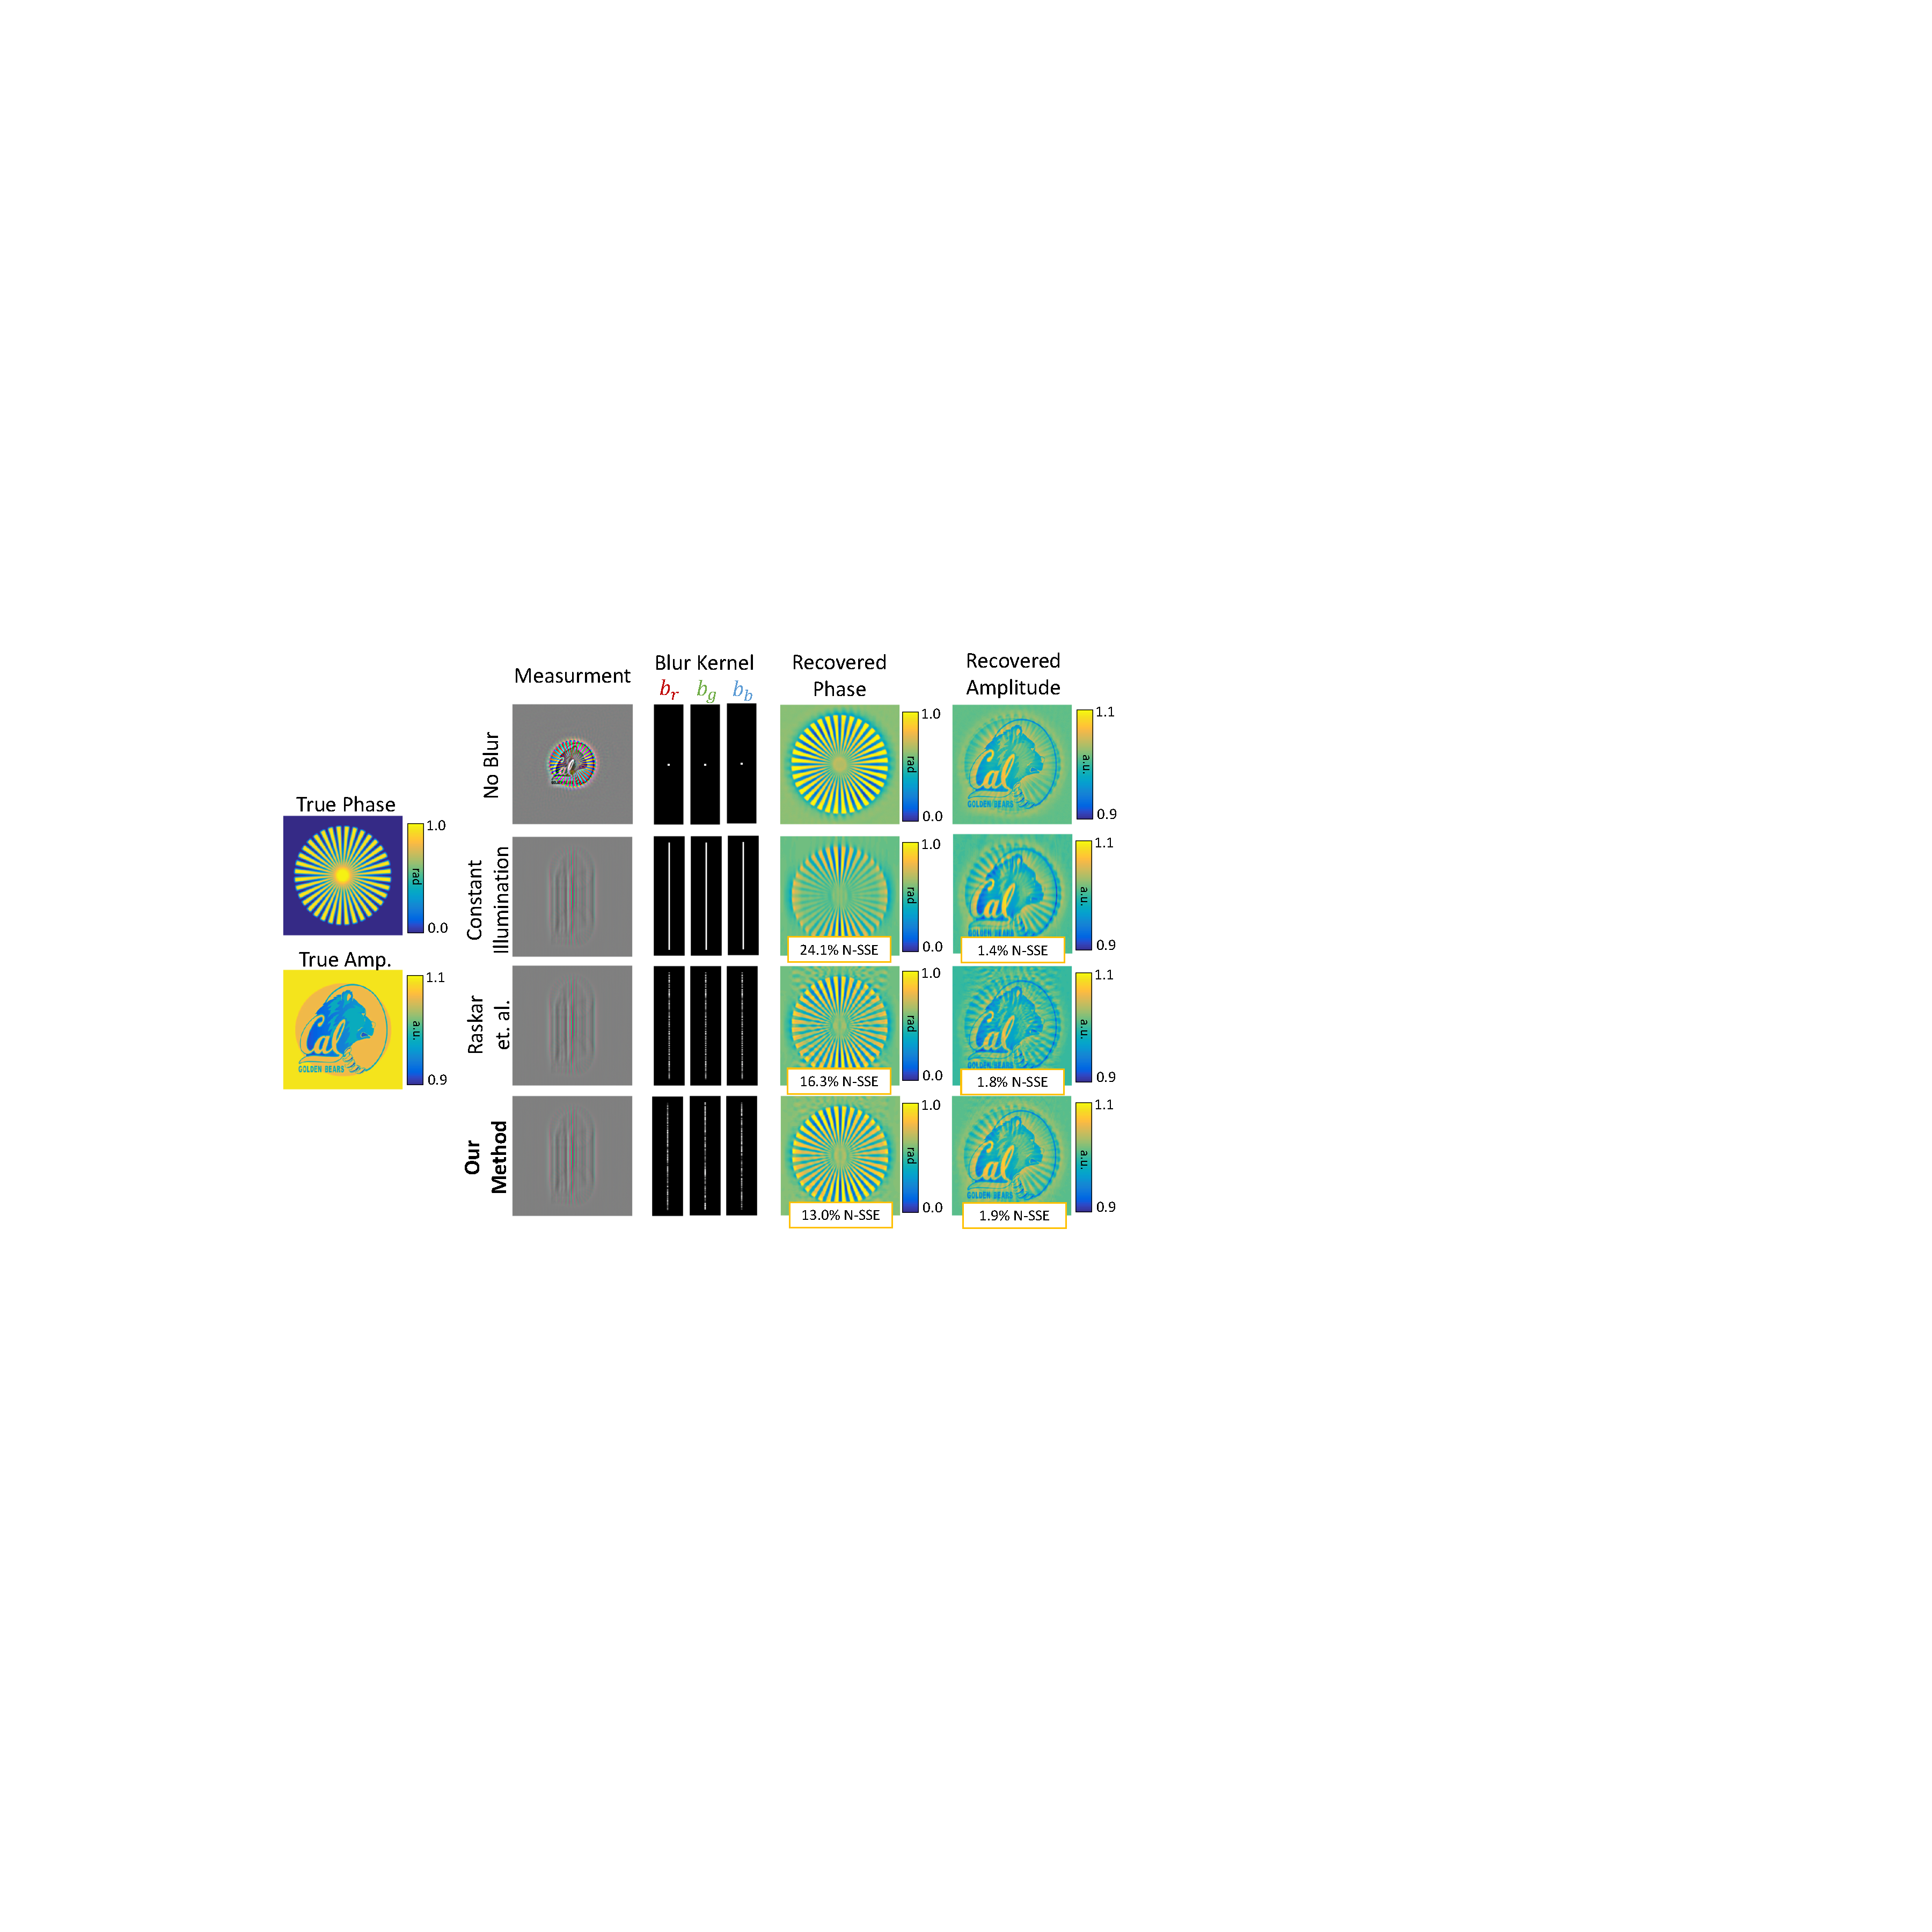
\includegraphics[width=0.9\textwidth]{deblur-fig3.pdf}
\caption{\label{fig:deblurSimulation}
Simulation results for phase retrieval from blurred images. \textbf{Top Row}: Phase and amplitude retrieval of a stationary sample. This serves as our best-case reconstruction for the blurred images. \textbf{Second Row}: Phase and amplitude retrieval of a blurred sample using constant illumination. This is the degenerate solution. \textbf{Third Row}: Deblur using a coded blur kernel as in the previous methods. The result improves significantly over the constant illumination case, but is still missing features in phase. \textbf{Fourth Row}: Deblur using our coded kernels}
\end{figure}

\section{Validation}
\subsection{Simulation}
Simulation results are shown in Fig. \ref{fig:deblurSimulation}. Here we show a static sample, deblurring without coded illumination, deblurring with the previous method (no spectral reference), and deblurring using our method, which accounts for the optical system transfer function. In this simulation we note that the normalized sum-squared error (N-SSE) in phase is reduced significantly in our method. The amplitude N-SSE did increase slightly using our method, which is likely due to the fact that we used the phase WOTF for generating our blur kernels instead of amplitude. The choice of which WOTF to use could be application-dependent.

\subsection{Experimental Results}

Our system consists of a commercial Nikon AZ100 microscope using a 1$\times$ 0.10 NA objective, a Bayer-patterned SCMOS camera (PCO.edge 5.5), an XY stage with linear encoders, (Prior H117), and illumination from 23 multi-channel LEDs (Jameco 2128500) arranged in a hexagonal pattern using a laser-cut holder for positioning. The LEDs were placed approximately 160mm from the sample to match the spacing such that the outer LEDs illuminate the sample from angles just inside of the NA of the microscope. This is done to ensure maximum phase contrast and bandwidth (resolution) of the system. The LEDs are controlled using a Teensy 3.2 microcontroller, which can be dynamically programmed. Camera exposures, stage movement, and illumination modulation are controlled using open-looped feedback with 5ms synchronization resolution, limited by the update speed of the LED array. This system is shown in Fig. \ref{fig:deblurSystem}.

\begin{figure}[ph]
\centering
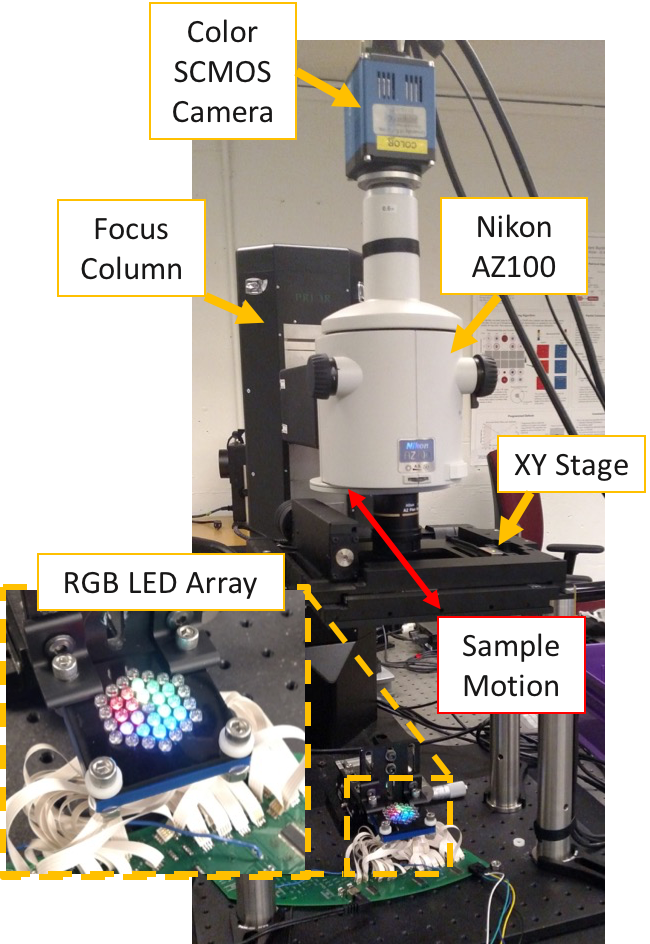
\includegraphics[width=0.8\textwidth]{deblur-fig5.png}
\caption{\label{fig:deblurSystem}
Experimental setup for motion deblurring. The tri-color LED array provides fast illumination coding in time, angle, and color. The LED array can be programmed dynamically using a Teensy micro-controller and has a maximum update speed of approximately 250 Hz. The LED array is synchronized with the linear motion stage and camera in hardware to provide precise system synchronization.}
\end{figure}

Our forward model considers the case where our LED illumination is incoherent and discrete, both spatially and temporally. We assume each emitter has three coincident emitters for Red ($\bar{\lambda} = 625$), Green ($\bar{\lambda} = 525$), and Blue ($\bar{\lambda} = 470$), wavelengths, which propagate through the optical system independently of each other and are detected separately by the bayer filter of our color camera. We assume a sample which is non-dispersive and unstained. A velocity of 25mm per second was used for sample movement, but this could be increased by improving hardware synchronization. Blur kernels were calculated using the calibrated phase WOTFs for each color channel separately, considering the spacing of k-space due to wavelength.

Experimental reconstructions are shown in Fig. \ref{fig:deblurResults}. To test our method, we used a micro-lens array (Fresnel-Tech 605) as our sample due to it's well-defined geometry. Fig. \ref{fig:deblurResults} shows reconstructions for the static case, previous method, and our method. While the sample amplitude is relatively unchanged, the phase reconstructions clearly show that accounting for the spectral reference provides better results than optimizing the blur kernel alone. This supports our claim that image degradation from blurring can be reduced significantly, but not eliminated, using our method.

\begin{figure}[ph]
\centering
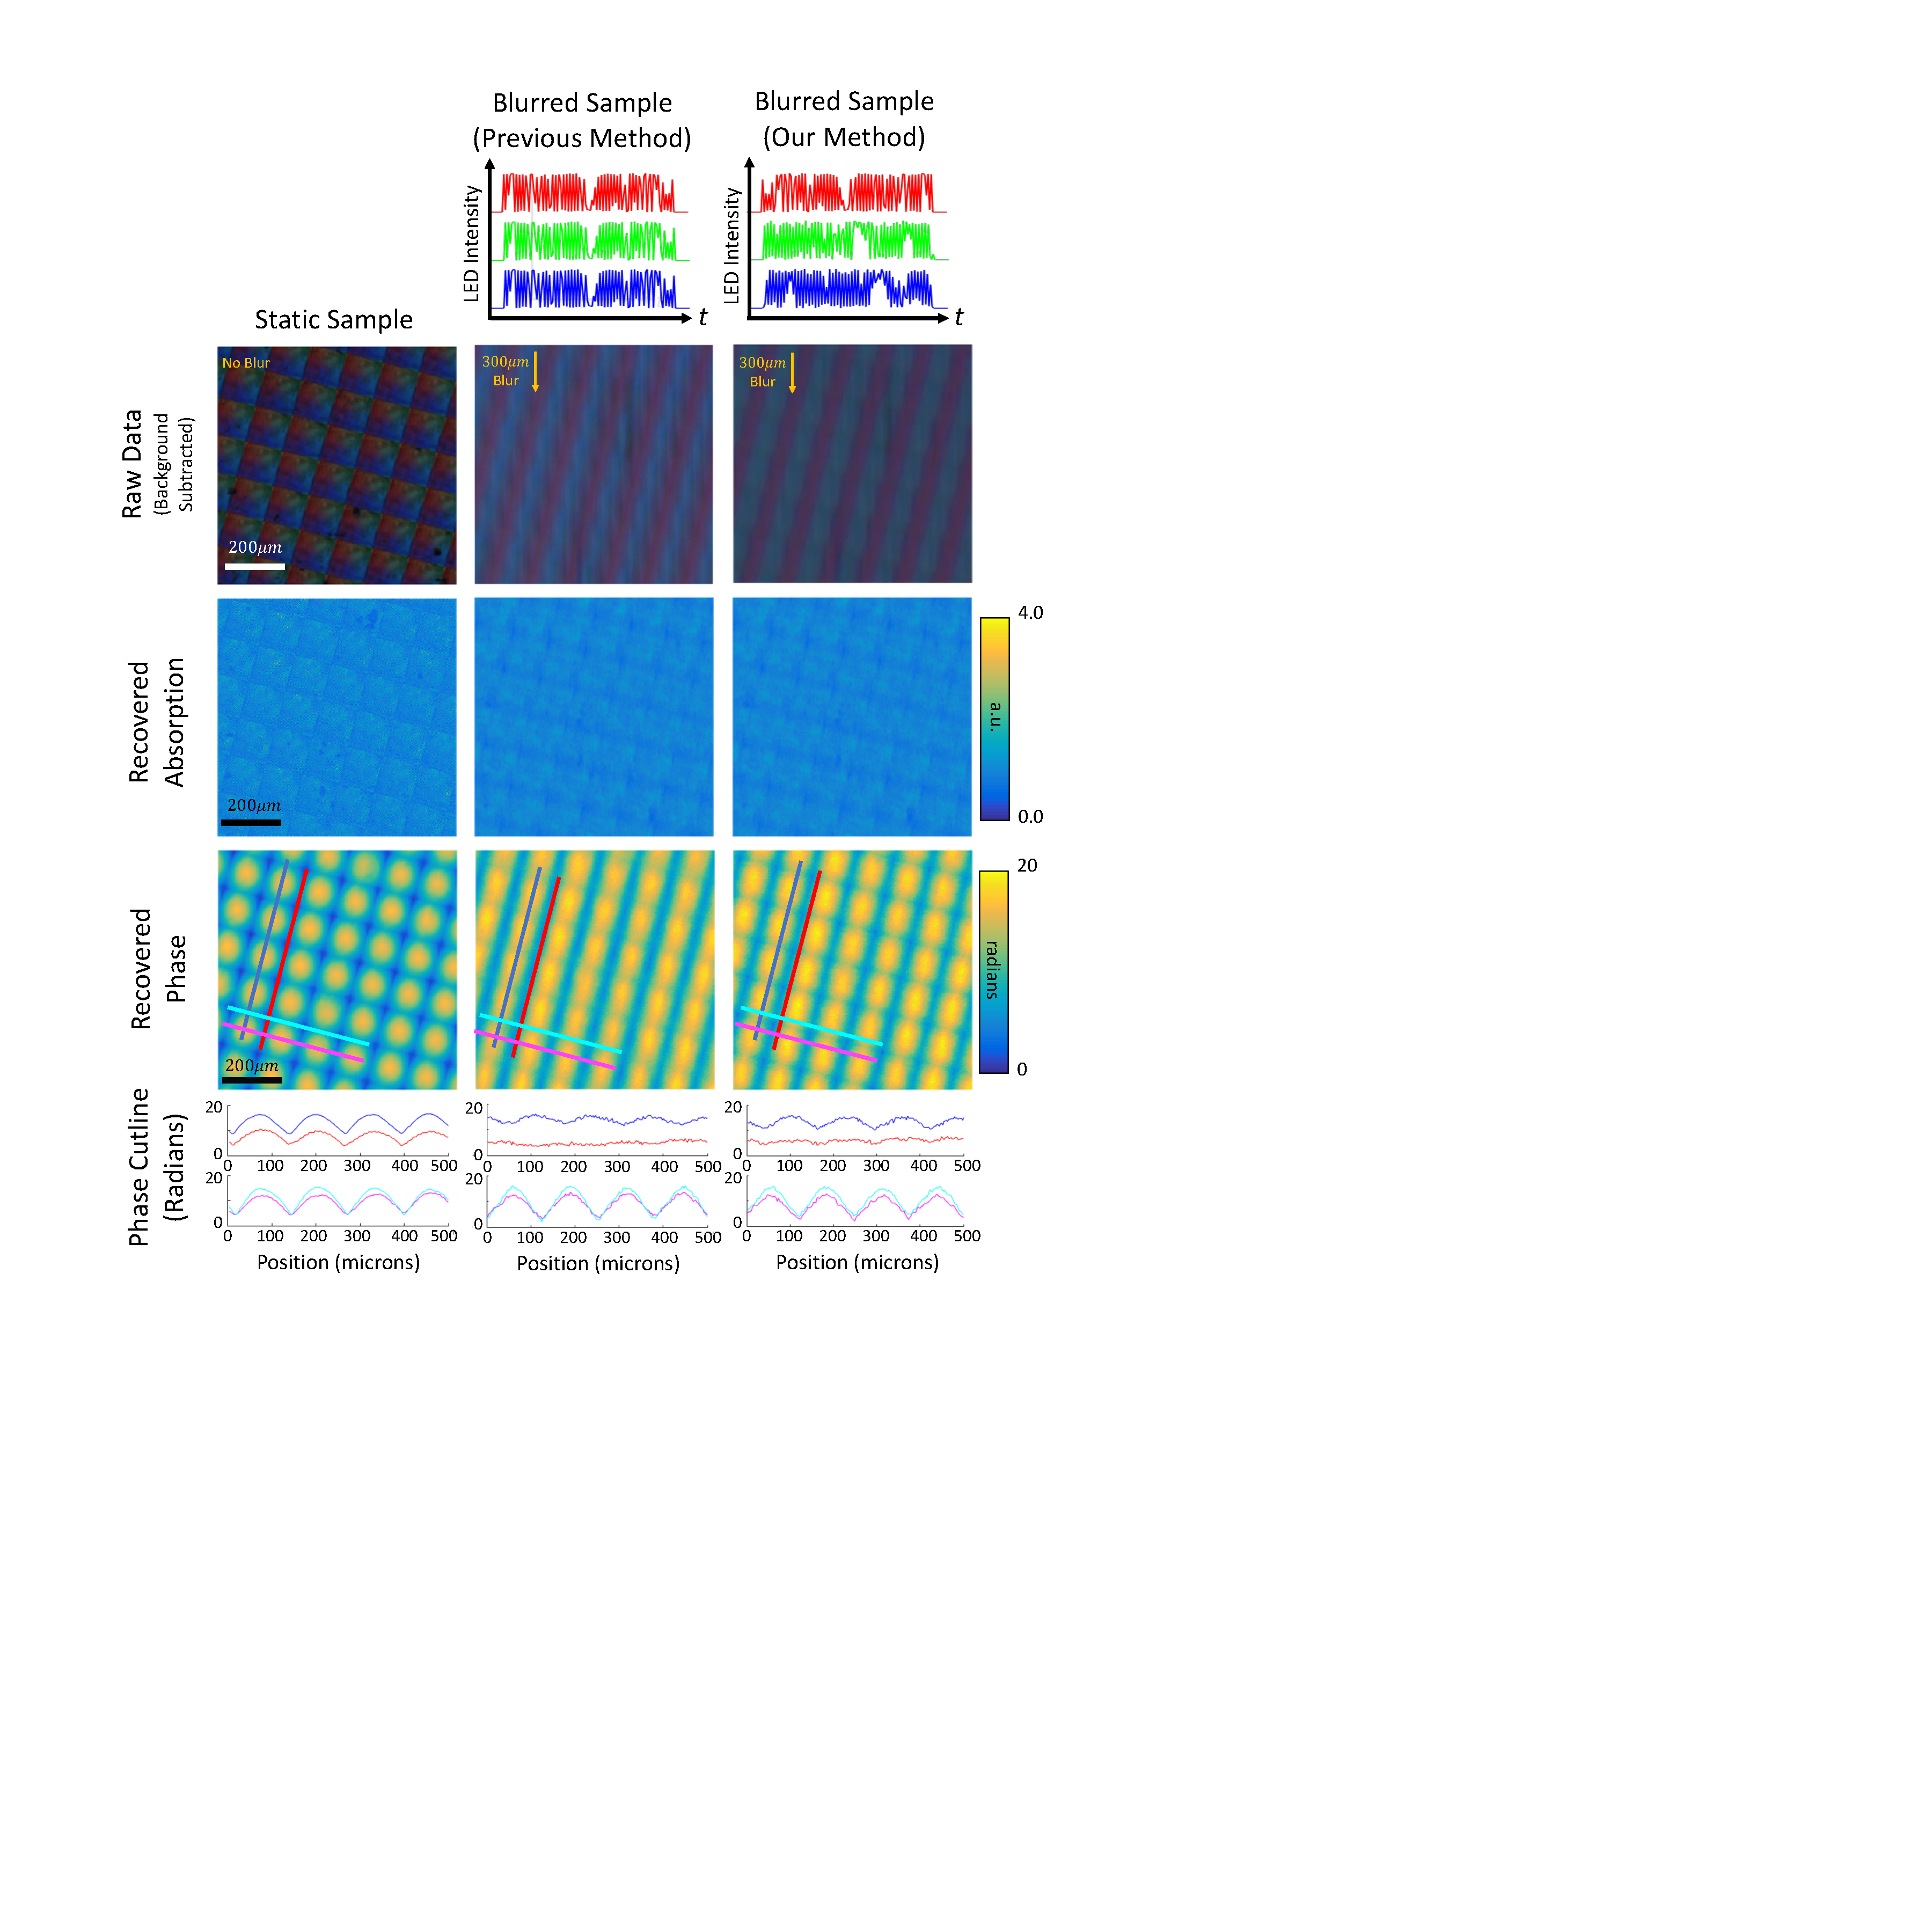
\includegraphics[width=0.8\textwidth]{deblur-fig4.pdf}
\caption{\label{fig:deblurResults}
Experimental results for motion deblur of a moving sample (Fresnel Technologies 605 micro-lens array).}
\end{figure}
